%%%%%%%%%%%%%%%%%%%%%%%%%%%%%%%%%%%%%%%%%
% The Legrand Orange Book
% LaTeX Template
% Version 1.4 (12/4/14)
%
% This template has been downloaded from:
% http://www.LaTeXTemplates.com
%
% Original author:
% Mathias Legrand (legrand.mathias@gmail.com)
%
% License:
% CC BY-NC-SA 3.0 (http://creativecommons.org/licenses/by-nc-sa/3.0/)
%
% Compiling this template:
% This template uses biber for its bibliography and makeindex for its index.
% When you first open the template, compile it from the command line with the 
% commands below to make sure your LaTeX distribution is configured correctly:
%
% 1) pdflatex main
% 2) makeindex main.idx -s StyleInd.ist
% 3) biber main
% 4) pdflatex main x 2
%
% After this, when you wish to update the bibliography/index use the appropriate
% command above and make sure to compile with pdflatex several times 
% afterwards to propagate your changes to the document.
%
% This template also uses a number of packages which may need to be
% updated to the newest versions for the template to compile. It is strongly
% recommended you update your LaTeX distribution if you have any
% compilation errors.
%
% Important note:
% Chapter heading images should have a 2:1 width:height ratio,
% e.g. 920px width and 460px height.
%
%%%%%%%%%%%%%%%%%%%%%%%%%%%%%%%%%%%%%%%%%

%----------------------------------------------------------------------------------------
%	PACKAGES AND OTHER DOCUMENT CONFIGURATIONS
%----------------------------------------------------------------------------------------

\documentclass[11pt,fleqn]{book} % Default font size and left-justified equations

\usepackage[top=3cm,bottom=3cm,left=3.2cm,right=3.2cm,headsep=10pt,a4paper]{geometry} % Page margins

\usepackage[table]{xcolor} % Required for specifying colors by name
\definecolor{heig}{RGB}{162,41,50} % Define the orange color used for highlighting throughout the book

% Font Settings
\usepackage{avant} % Use the Avantgarde font for headings
%\usepackage{times} % Use the Times font for headings
\usepackage{mathptmx} % Use the Adobe Times Roman as the default text font together with math symbols from the Sym­bol, Chancery and Com­puter Modern fonts

\usepackage{microtype} % Slightly tweak font spacing for aesthetics
\usepackage[utf8]{inputenc} % Required for including letters with accents
\usepackage[T1]{fontenc} % Use 8-bit encoding that has 256 glyphs

\usepackage{multirow,tabularx,longtable,booktabs,multirow}
\newcolumntype{Y}{>{\centering\arraybackslash}X}
\renewcommand{\arraystretch}{2}

\usepackage{arydshln}

% Bibliography
%\usepackage[style=alphabetic,sorting=nyt,sortcites=true,autopunct=true,babel=hyphen,hyperref=true,abbreviate=false,backref=true,backend=biber]{biblatex}
%\addbibresource{bibliography.bib} % BibTeX bibliography file
%\defbibheading{bibempty}{}

% Index
\usepackage{calc} % For simpler calculation - used for spacing the index letter headings correctly
\usepackage{makeidx} % Required to make an index
\makeindex % Tells LaTeX to create the files required for indexing

%----------------------------------------------------------------------------------------

%----------------------------------------------------------------------------------------
%	VARIOUS REQUIRED PACKAGES
%----------------------------------------------------------------------------------------

\usepackage{titlesec} % Allows customization of titles

\usepackage{graphicx} % Required for including pictures
\graphicspath{{images/}} % Specifies the directory where pictures are stored

\usepackage{lipsum} % Inserts dummy text

\usepackage{tikz} % Required for drawing custom shapes

\usepackage[francais]{babel} % English language/hyphenation
\frenchbsetup{StandardItemizeEnv=true}
\selectlanguage{francais}

\usepackage{enumitem} % Customize lists
%\setlist{nolistsep} % Reduce spacing between bullet points and numbered lists

\usepackage{booktabs} % Required for nicer horizontal rules in tables

\usepackage{eso-pic} % Required for specifying an image background in the title page

%----------------------------------------------------------------------------------------
%	MAIN TABLE OF CONTENTS
%----------------------------------------------------------------------------------------

\usepackage{titletoc} % Required for manipulating the table of contents

\contentsmargin{0cm} % Removes the default margin
% Chapter text styling
\titlecontents{chapter}[1.25cm] % Indentation
{\addvspace{15pt}\large\sffamily\bfseries} % Spacing and font options for chapters
{\color{heig!60}\contentslabel[\Large\thecontentslabel]{1.25cm}\color{heig}} % Chapter number
{}  
{\color{heig!60}\normalsize\sffamily\bfseries\;\titlerule*[.5pc]{.}\;\thecontentspage} % Page number
% Section text styling
\titlecontents{section}[1.25cm] % Indentation
{\addvspace{5pt}\sffamily\bfseries} % Spacing and font options for sections
{\contentslabel[\thecontentslabel]{1.25cm}} % Section number
{}
{\sffamily\hfill\color{black}\thecontentspage} % Page number
[]
% Subsection text styling
\titlecontents{subsection}[1.25cm] % Indentation
{\addvspace{1pt}\sffamily\small} % Spacing and font options for subsections
{\contentslabel[\thecontentslabel]{1.25cm}} % Subsection number
{}
{\sffamily\;\titlerule*[.5pc]{.}\;\thecontentspage} % Page number
[] 

%----------------------------------------------------------------------------------------
%	MINI TABLE OF CONTENTS IN CHAPTER HEADS
%----------------------------------------------------------------------------------------

% Section text styling
\titlecontents{lsection}[0em] % Indendating
{\footnotesize\sffamily} % Font settings
{}
{}
{}

% Subsection text styling
\titlecontents{lsubsection}[.5em] % Indentation
{\normalfont\footnotesize\sffamily} % Font settings
{}
{}
{}
 
%----------------------------------------------------------------------------------------
%	PAGE HEADERS
%----------------------------------------------------------------------------------------

\usepackage{fancyhdr} % Required for header and footer configuration

\pagestyle{fancy}
\renewcommand{\chaptermark}[1]{\markboth{\sffamily\normalsize\bfseries\chaptername\ \thechapter.\ #1}{}} % Chapter text font settings
\renewcommand{\sectionmark}[1]{\markright{\sffamily\normalsize\thesection\hspace{5pt}#1}{}} % Section text font settings
\fancyhf{} \fancyhead[LE,RO]{\sffamily\normalsize\thepage} % Font setting for the page number in the header
\fancyhead[LO]{\rightmark} % Print the nearest section name on the left side of odd pages
\fancyhead[RE]{\leftmark} % Print the current chapter name on the right side of even pages
\renewcommand{\headrulewidth}{0.5pt} % Width of the rule under the header
\addtolength{\headheight}{2.5pt} % Increase the spacing around the header slightly
\renewcommand{\footrulewidth}{0pt} % Removes the rule in the footer
\fancypagestyle{plain}{\fancyhead{}\renewcommand{\headrulewidth}{0pt}} % Style for when a plain pagestyle is specified

% Removes the header from odd empty pages at the end of chapters
\makeatletter
\renewcommand{\cleardoublepage}{
\clearpage\ifodd\c@page\else
\hbox{}
\vspace*{\fill}
\thispagestyle{empty}
\newpage
\fi}

%----------------------------------------------------------------------------------------
%	THEOREM STYLES
%----------------------------------------------------------------------------------------

\usepackage{amsmath,amsfonts,amssymb,amsthm} % For math equations, theorems, symbols, etc

\newcommand{\intoo}[2]{\mathopen{]}#1\,;#2\mathclose{[}}
\newcommand{\ud}{\mathop{\mathrm{{}d}}\mathopen{}}
\newcommand{\intff}[2]{\mathopen{[}#1\,;#2\mathclose{]}}
\newtheorem{notation}{Notation}[chapter]

%%%%%%%%%%%%%%%%%%%%%%%%%%%%%%%%%%%%%%%%%%%%%%%%%%%%%%%%%%%%%%%%%%%%%%%%%%%
%%%%%%%%%%%%%%%%%%%% dedicated to boxed/framed environements %%%%%%%%%%%%%%
%%%%%%%%%%%%%%%%%%%%%%%%%%%%%%%%%%%%%%%%%%%%%%%%%%%%%%%%%%%%%%%%%%%%%%%%%%%
\newtheoremstyle{ocrenumbox}% % Theorem style name
{0pt}% Space above
{0pt}% Space below
{\normalfont}% % Body font
{}% Indent amount
{\small\bf\sffamily\color{heig}}% % Theorem head font
{\;}% Punctuation after theorem head
{0.25em}% Space after theorem head
{\small\sffamily\color{heig}\thmname{#1}\nobreakspace\thmnumber{\@ifnotempty{#1}{}\@upn{#2}}% Theorem text (e.g. Theorem 2.1)
\thmnote{\nobreakspace\the\thm@notefont\sffamily\bfseries\color{black}---\nobreakspace#3.}} % Optional theorem note
\renewcommand{\qedsymbol}{$\blacksquare$}% Optional qed square

\newtheoremstyle{blacknumex}% Theorem style name
{5pt}% Space above
{5pt}% Space below
{\normalfont}% Body font
{} % Indent amount
{\small\bf\sffamily}% Theorem head font
{\;}% Punctuation after theorem head
{0.25em}% Space after theorem head
{\small\sffamily{\tiny\ensuremath{\blacksquare}}\nobreakspace\thmname{#1}\nobreakspace\thmnumber{\@ifnotempty{#1}{}\@upn{#2}}% Theorem text (e.g. Theorem 2.1)
\thmnote{\nobreakspace\the\thm@notefont\sffamily\bfseries---\nobreakspace#3.}}% Optional theorem note

\newtheoremstyle{blacknumbox} % Theorem style name
{0pt}% Space above
{0pt}% Space below
{\normalfont}% Body font
{}% Indent amount
{\small\bf\sffamily}% Theorem head font
{\;}% Punctuation after theorem head
{0.25em}% Space after theorem head
{\small\sffamily\thmname{#1}\nobreakspace\thmnumber{\@ifnotempty{#1}{}\@upn{#2}}% Theorem text (e.g. Theorem 2.1)
\thmnote{\nobreakspace\the\thm@notefont\sffamily\bfseries---\nobreakspace#3.}}% Optional theorem note

%%%%%%%%%%%%%%%%%%%%%%%%%%%%%%%%%%%%%%%%%%%%%%%%%%%%%%%%%%%%%%%%%%%%%%%%%%%
%%%%%%%%%%%%% dedicated to non-boxed/non-framed environements %%%%%%%%%%%%%
%%%%%%%%%%%%%%%%%%%%%%%%%%%%%%%%%%%%%%%%%%%%%%%%%%%%%%%%%%%%%%%%%%%%%%%%%%%
\newtheoremstyle{ocrenum}% % Theorem style name
{5pt}% Space above
{5pt}% Space below
{\normalfont}% % Body font
{}% Indent amount
{\small\bf\sffamily\color{heig}}% % Theorem head font
{\;}% Punctuation after theorem head
{0.25em}% Space after theorem head
{\small\sffamily\color{heig}\thmname{#1}\nobreakspace\thmnumber{\@ifnotempty{#1}{}\@upn{#2}}% Theorem text (e.g. Theorem 2.1)
\thmnote{\nobreakspace\the\thm@notefont\sffamily\bfseries\color{black}---\nobreakspace#3.}} % Optional theorem note
\renewcommand{\qedsymbol}{$\blacksquare$}% Optional qed square
\makeatother

% Defines the theorem text style for each type of theorem to one of the three styles above
\newcounter{dummy} 
\numberwithin{dummy}{section}
\theoremstyle{ocrenumbox}
\newtheorem{theoremeT}[dummy]{Theorem}
\newtheorem{problem}{Problem}[chapter]
\newtheorem{exerciseT}{Exercise}[chapter]
\theoremstyle{blacknumex}
\newtheorem{exampleT}{Example}[chapter]
\theoremstyle{blacknumbox}
\newtheorem{vocabulary}{Vocabulary}[chapter]
\newtheorem{definitionT}{Definition}[section]
\newtheorem{corollaryT}[dummy]{Corollary}
\newtheorem{infoT}[dummy]{Information}
\theoremstyle{ocrenum}
\newtheorem{proposition}[dummy]{Proposition}

%----------------------------------------------------------------------------------------
%	DEFINITION OF COLORED BOXES
%----------------------------------------------------------------------------------------

\RequirePackage[framemethod=default]{mdframed} % Required for creating the theorem, definition, exercise and corollary boxes

% Theorem box
\newmdenv[skipabove=7pt,
skipbelow=7pt,
backgroundcolor=black!5,
linecolor=heig,
innerleftmargin=5pt,
innerrightmargin=5pt,
innertopmargin=5pt,
leftmargin=0cm,
rightmargin=0cm,
innerbottommargin=5pt]{tBox}

% Exercise box	  
\newmdenv[skipabove=7pt,
skipbelow=7pt,
rightline=false,
leftline=true,
topline=false,
bottomline=false,
backgroundcolor=heig!10,
linecolor=heig,
innerleftmargin=5pt,
innerrightmargin=5pt,
innertopmargin=5pt,
innerbottommargin=5pt,
leftmargin=0cm,
rightmargin=0cm,
linewidth=4pt]{eBox}	

% Definition box
\newmdenv[skipabove=7pt,
skipbelow=7pt,
rightline=false,
leftline=true,
topline=false,
bottomline=false,
linecolor=heig,
innerleftmargin=5pt,
innerrightmargin=5pt,
innertopmargin=0pt,
leftmargin=0cm,
rightmargin=0cm,
linewidth=4pt,
innerbottommargin=0pt]{dBox}	

% Corollary box
\newmdenv[skipabove=7pt,
skipbelow=7pt,
rightline=false,
leftline=true,
topline=false,
bottomline=false,
linecolor=gray,
backgroundcolor=black!5,
innerleftmargin=5pt,
innerrightmargin=5pt,
innertopmargin=5pt,
leftmargin=0cm,
rightmargin=0cm,
linewidth=4pt,
innerbottommargin=5pt]{cBox}

% Exercise box	  
\newmdenv[skipabove=7pt,
skipbelow=7pt,
rightline=false,
leftline=true,
topline=false,
bottomline=false,
backgroundcolor=cyan!10,
linecolor=cyan,
innerleftmargin=5pt,
innerrightmargin=5pt,
innertopmargin=5pt,
innerbottommargin=5pt,
leftmargin=0cm,
rightmargin=0cm,
linewidth=4pt]{infoBox}	

% Creates an environment for each type of theorem and assigns it a theorem text style from the "Theorem Styles" section above and a colored box from above
\newenvironment{theorem}{\begin{tBox}\begin{theoremeT}}{\end{theoremeT}\end{tBox}}
\newenvironment{exercise}{\begin{eBox}\begin{exerciseT}}{\hfill{\color{heig}\tiny\ensuremath{\blacksquare}}\end{exerciseT}\end{eBox}}				  
\newenvironment{definition}{\begin{dBox}\begin{definitionT}}{\end{definitionT}\end{dBox}}	
\newenvironment{example}{\begin{exampleT}}{\hfill{\tiny\ensuremath{\blacksquare}}\end{exampleT}}		
\newenvironment{corollary}{\begin{cBox}\begin{corollaryT}}{\end{corollaryT}\end{cBox}}
\newenvironment{info}{\begin{infoBox}\begin{infoT}}{\end{infoT}\end{infoBox}}

%----------------------------------------------------------------------------------------
%	REMARK ENVIRONMENT
%----------------------------------------------------------------------------------------

\newenvironment{remark}{\par\vspace{10pt}\small % Vertical white space above the remark and smaller font size
\begin{list}{}{
\leftmargin=35pt % Indentation on the left
\rightmargin=25pt}\item\ignorespaces % Indentation on the right
\makebox[-2.5pt]{\begin{tikzpicture}[overlay]
\node[draw=heig!60,line width=1pt,circle,fill=heig!25,font=\sffamily\bfseries,inner sep=2pt,outer sep=0pt] at (-15pt,0pt){\textcolor{heig}{R}};\end{tikzpicture}} % Orange R in a circle
\advance\baselineskip -1pt}{\end{list}\vskip5pt} % Tighter line spacing and white space after remark

%----------------------------------------------------------------------------------------
%	SECTION NUMBERING IN THE MARGIN
%----------------------------------------------------------------------------------------

\makeatletter
\renewcommand{\@seccntformat}[1]{\llap{\textcolor{heig}{\csname the#1\endcsname}\hspace{1em}}}
\renewcommand{\section}{\@startsection{section}{1}{\z@}
{-4ex \@plus -1ex \@minus -.4ex}
{1ex \@plus.2ex }
{\normalfont\large\sffamily\bfseries}}
\renewcommand{\subsection}{\@startsection {subsection}{2}{\z@}
{-3ex \@plus -0.1ex \@minus -.4ex}
{0.5ex \@plus.2ex }
{\normalfont\sffamily\bfseries}}
\renewcommand{\subsubsection}{\@startsection {subsubsection}{3}{\z@}
{-2ex \@plus -0.1ex \@minus -.2ex}
{.2ex \@plus.2ex }
{\normalfont\small\sffamily\bfseries}}                      
\renewcommand\paragraph{\@startsection{paragraph}{4}{\z@}
{-2ex \@plus-.2ex \@minus .2ex}
{.1ex}
{\normalfont\small\sffamily\bfseries}}

%----------------------------------------------------------------------------------------
%	HYPERLINKS IN THE DOCUMENTS
%----------------------------------------------------------------------------------------

% For an unclear reason, the package should be loaded now and not later
\usepackage{hyperref}
\hypersetup{hidelinks, colorlinks=true, breaklinks=true, linkcolor=, urlcolor=heig,  bookmarksopen=false, pdftitle={Title}, pdfauthor={Author}}

%----------------------------------------------------------------------------------------
%	CHAPTER HEADINGS
%----------------------------------------------------------------------------------------

% The set-up below should be (sadly) manually adapted to the overall margin page septup controlled by the geometry package loaded in the main.tex document. It is possible to implement below the dimensions used in the goemetry package (top,bottom,left,right)... TO BE DONE

\newcommand{\thechapterimage}{}
\newcommand{\chapterimage}[1]{\renewcommand{\thechapterimage}{#1}}

% Numbered chapters with mini tableofcontents
\def\thechapter{\arabic{chapter}}
\def\@makechapterhead#1{
\thispagestyle{empty}
{\centering \normalfont\sffamily
\ifnum \c@secnumdepth >\m@ne
\if@mainmatter
\startcontents
\begin{tikzpicture}[remember picture,overlay]
\node at (current page.north west)
{\begin{tikzpicture}[remember picture,overlay]
\node[anchor=north west,inner sep=0pt] at (0,0) {\includegraphics[width=\paperwidth]{\thechapterimage}};
%%%%%%%%%%%%%%%%%%%%%%%%%%%%%%%%%%%%%%%%%%%%%%%%%%%%%%%%%%%%%%%%%%%%%%%%%%%%%%%%%%%%%
% Commenting the 3 lines below removes the small contents box in the chapter heading
%\fill[color=heig!10!white,opacity=.6] (1cm,0) rectangle (8cm,-7cm);
%\node[anchor=north west] at (1.1cm,.35cm) {\parbox[t][8cm][t]{6.5cm}{\huge\bfseries\flushleft \printcontents{l}{1}{\setcounter{tocdepth}{2}}}};
\draw[anchor=west] (5cm,-9cm) node [rounded corners=20pt,fill=heig!10!white,text opacity=1,draw=heig,draw opacity=1,line width=1.5pt,fill opacity=.6,inner sep=12pt]{\huge\sffamily\bfseries\textcolor{black}{\thechapter. #1\strut\makebox[22cm]{}}};
%%%%%%%%%%%%%%%%%%%%%%%%%%%%%%%%%%%%%%%%%%%%%%%%%%%%%%%%%%%%%%%%%%%%%%%%%%%%%%%%%%%%%
\end{tikzpicture}};
\end{tikzpicture}}
\par\vspace*{230\p@}
\fi
\fi}

% Unnumbered chapters without mini tableofcontents (could be added though) 
\def\@makeschapterhead#1{
\thispagestyle{empty}
{\centering \normalfont\sffamily
\ifnum \c@secnumdepth >\m@ne
\if@mainmatter
\begin{tikzpicture}[remember picture,overlay]
\node at (current page.north west)
{\begin{tikzpicture}[remember picture,overlay]
\node[anchor=north west,inner sep=0pt] at (0,0) {\includegraphics[width=\paperwidth]{\thechapterimage}};
\draw[anchor=west] (5cm,-9cm) node [rounded corners=20pt,fill=heig!10!white,fill opacity=.6,inner sep=12pt,text opacity=1,draw=heig,draw opacity=1,line width=1.5pt]{\huge\sffamily\bfseries\textcolor{black}{#1\strut\makebox[22cm]{}}};
\end{tikzpicture}};
\end{tikzpicture}}
\par\vspace*{230\p@}
\fi
\fi
}
\makeatother % Insert the commands.tex file which contains the majority of the structure behind the template

\selectlanguage{francais}
\setlength{\parindent}{0pt}
\setlength{\parskip}{1ex plus0.2ex minus0.2ex}

\renewcommand{\baselinestretch}{1.1}
\renewcommand{\labelitemi}{$\triangleright$}

\begin{document}

%\maketitle
%\tableofcontents

%----------------------------------------------------------------------------------------
%	TITLE PAGE
%----------------------------------------------------------------------------------------

\begingroup
\thispagestyle{empty}
\centering
\vspace*{9cm}
\par\normalfont\fontsize{35}{35}\sffamily\selectfont

Manuel d'utilisation \par % Book title

\vspace*{1cm}
{\Huge Slyum 5}\par % Author name
\endgroup

%----------------------------------------------------------------------------------------
%	TABLE OF CONTENTS
%----------------------------------------------------------------------------------------

\chapterimage{no_chapter_image.png} % Table of contents heading image

\pagestyle{empty} % No headers

\tableofcontents % Print the table of contents itself

\cleardoublepage % Forces the first chapter to start on an odd page so it's on the right

\pagestyle{fancy} % Print headers again

\chapter{Présentation générale}

\section*{Qu'est-ce que Slyum}

\texttt{Slyum} est un éditeur de diagramme de classes UML (Unified Modeling Language) conçu pour être simple à prendre en main et à utiliser. La figure ~\ref{img:main_screen} représente l'affichage classique de Slyum.

\begin{figure}[h]
	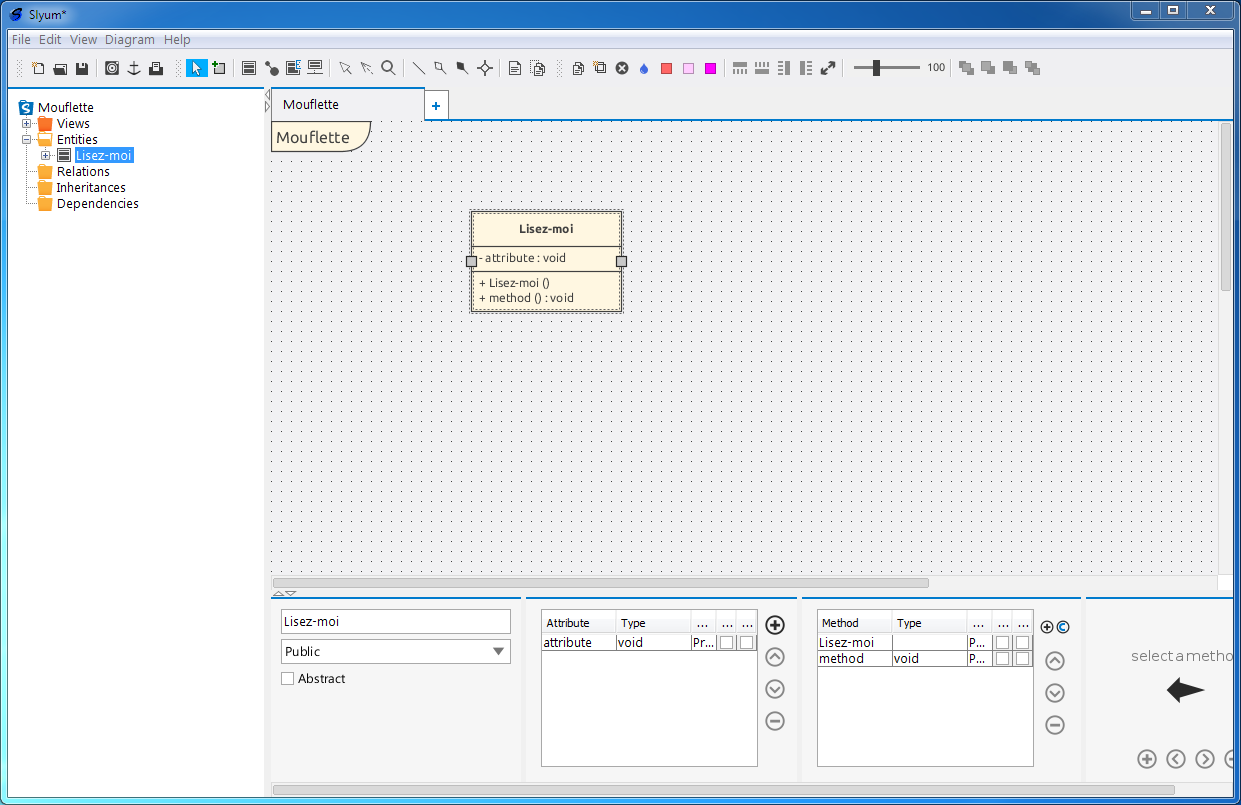
\includegraphics[width=\textwidth]{images/slyum-window.png}
	\caption{Capture d'écran de Slyum}
	\label{img:main_screen}
\end{figure}

\section*{Remarques, questions et bugs (à revoir)}

Pour tout report de problème, proposition d'amélioration ou de remarque, merci de vous rendre à l'adresse suivante:
https://github.com/HEIG-GAPS/slyum/issues.
Depuis cette interface, vous pouvez également voir les problème déjà reportés. Merci de vous assurez que le problème n'existe pas déjà avant d'en reporter un.

\chapter{Utilisation de Slyum}

La figure ~\ref{img:main_screen} montre l'interface de Slyum dans son entier. La partie de gauche liste sous forme d'arbre l'ensemble des éléments du projet actuellement ouvert. La partie du bas affiche des propriétés pour l'élément actuellement sélectionné du diagramme. Et enfin, la partie centrale correspond aux diagrammes de classes UML actuellement ouverts.

\section{Créer un diagramme de classes}

\begin{figure}[h]
	\centering	
	\begin{minipage}[c]{0.54\textwidth}
		La partie centrale (figure ~\ref{img:partie_centrale}) permet de créer le diagramme de classes de manière graphique en disposant les différents éléments sur la zone prévue à cet effet. Un projet peut contenir plusieurs diagrammes (section \ref{sec:vues} Vues) se basant sur la même structure de données établie. Dans le cas où plusieurs vues sont ouvertes, il est possible de change celle qui est affichée en changeant d'onglets.
	\end{minipage}
	\begin{minipage}{0.45\textwidth}
		\flushright
		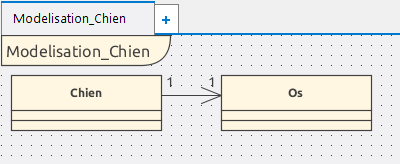
\includegraphics[width=0.95\linewidth]{images/partie_centrale.png}
		\caption{Diagramme de classes}
		\label{img:partie_centrale}
	\end{minipage}
\end{figure}

\section{Liste des éléments}
La partie de gauche de Slyum est une représentation sous forme d'arbre de tous les éléments UML existants dans le projet actuellement ouvert.

Les éléments sont classés dans cinq catégories représentées chacune par un noeud principal de l'arbre. Ces catégories sont Views (\ref{sec:vues}), Entities (\ref{sec:entites}), Relations (\ref{sec:relations}), Inheritances (\ref{sec:relations}), Dependencies (\ref{sec:relations}).

element en rouge

glisser déplacer

menu contextuel

sélection


\section{Propriétés des éléments}

\newmdenv[topline=false,leftline=false,bottomline=false]{rightborder}

\chapter{Fonctionnalités (à revoir)}

\section*{Composants (à revoir)}

Cette section liste à quoi correspond les différents icônes pouvant être rencontrés dans Slyum ainsi que le chapitre qui leur est associé.

\subsection*{Composants de Slyum}


% Projets
\begin{minipage}[c]{.2\textwidth}
	\begin{rightborder}\begin{tabular}{cc}
		
\includegraphics{images/icon/open.png} &
		
\includegraphics{images/icon/new.png} \\
		
\includegraphics{images/icon/save.png} &
		
\includegraphics{images/icon/print.png} \\
		
\includegraphics{images/icon/pdf-16.png} &
		... \\
	\end{tabular}\end{rightborder}
\end{minipage}
\begin{minipage}[c]{.1\textwidth}\end{minipage}
\begin{minipage}[c]{.6\textwidth}
	\textbf{Projet} \\
	Représente les outils pour gérer les projets, les exportations ou encore les impressions.
\end{minipage}
\begin{minipage}[c]{.1\textwidth}
	\hfill
	p.{\LARGE \pageref{sec:projet}}
\end{minipage}

% Vues
\begin{minipage}[c]{.2\textwidth}
    \begin{rightborder}\begin{tabular}{cc}
		
\includegraphics{images/icon/element-view.png} &
		
\includegraphics{images/icon/element-view-open.png} \\
		
\includegraphics{images/icon/element-view-add.png} &
		
\includegraphics{images/icon/element-view-delete.png} \\
    \end{tabular}\end{rightborder}
\end{minipage}
\begin{minipage}[c]{.1\textwidth}\end{minipage}
\begin{minipage}[c]{.6\textwidth}
    \textbf{Vues} \\
    Représente une vue du projet. Permet de créer, ouvrir et supprimer des vues.
\end{minipage}
\begin{minipage}[c]{.1\textwidth}
    \hfill
    p.{\LARGE \pageref{sec:vues}}
\end{minipage}

\subsection*{Composants UML}

% Entités
\begin{minipage}[c]{.2\textwidth}
    \begin{rightborder}\begin{tabular}{cc}
        
\includegraphics{images/icon/class.png} &
        
\includegraphics{images/icon/interface.png} \\
        
\includegraphics{images/icon/enum.png} &
        
\includegraphics{images/icon/classAssoc.png} \\
    \end{tabular}\end{rightborder}
\end{minipage}
\begin{minipage}[c]{.1\textwidth}\end{minipage}
\begin{minipage}[c]{.6\textwidth}
    \textbf{Entités} \\
    Représente les différentes entités UML telles que les classes ou les interfaces.
\end{minipage}
\begin{minipage}[c]{.1\textwidth}
    \hfill
    p.{\LARGE \pageref{sec:entites}}
\end{minipage}

% Association
\begin{minipage}[c]{.2\textwidth}
    \begin{rightborder}\begin{tabular}{cc}
        
\includegraphics{images/icon/generalize.png} &
        
\includegraphics{images/icon/dependency.png} \\
        
\includegraphics{images/icon/association.png} &
        
\includegraphics{images/icon/aggregation.png} \\
        
\includegraphics{images/icon/composition.png} &
        
\includegraphics{images/icon/innerClass.png} \\
        \multicolumn{2}{c}{
\includegraphics[width=13px]{images/icon/multi.png}} \\
    \end{tabular}\end{rightborder}
\end{minipage}
\begin{minipage}[c]{.1\textwidth}\end{minipage}
\begin{minipage}[c]{.6\textwidth}
    \textbf{Relations} \\
    Représente les différentes relations entre entités UML telle que les associations, les aggrégations ou encore les héritages.
\end{minipage}
\begin{minipage}[c]{.1\textwidth}
    \hfill
    p.{\LARGE \pageref{sec:relations}}
\end{minipage}

% Notes
\begin{minipage}[c]{.2\textwidth}
	\begin{rightborder}\begin{tabular}{cc}
		
\includegraphics{images/icon/note.png} &
		
\includegraphics{images/icon/linkNote.png} \\
		\multicolumn{2}{c}{
\includegraphics{images/icon/multiNote.png}} \\
	\end{tabular}\end{rightborder}
\end{minipage}
\begin{minipage}[c]{.1\textwidth}\end{minipage}
\begin{minipage}[c]{.6\textwidth}
	\textbf{Notes} \\
	Représentation des notes. Permet de créer des notes sur le diagramme de classe.
\end{minipage}
\begin{minipage}[c]{.1\textwidth}
	\hfill
	p.{\LARGE \pageref{sec:notes}}
\end{minipage}

% Outils de personnalisation
\begin{minipage}[c]{.2\textwidth}
	\begin{rightborder}\begin{tabular}{cc}
		
\includegraphics{images/icon/pointer-grip.png} &
		
\includegraphics{images/icon/alignLeft.png} \\
		
\includegraphics{images/icon/delete.png} &
		
\includegraphics{images/icon/color.png} \\
		
\includegraphics{images/icon/top.png} &
		... \\
	\end{tabular}\end{rightborder}
\end{minipage}
\begin{minipage}[c]{.1\textwidth}\end{minipage}
\begin{minipage}[c]{.6\textwidth}
	\textbf{Outils de personnalisation} \\
	Représente les outils permettant de personnaliser et modifier les différents composants du diagramme.
\end{minipage}
\begin{minipage}[c]{.1\textwidth}
	\hfill
	p.{\LARGE \pageref{ch:outils}}
\end{minipage}

\chapter{Gestion de projet et vues}
\label{ch:gestion_projet}


\section{Projet}
\label{sec:projet}


\section{Vues}
\label{sec:vues}


\chapter{Composants UML}
\label{ch:composants_uml}

\section{Entités}
\label{sec:entites}

\section{Relations}
\label{sec:relations}

\section{Notes}
\label{sec:notes}

\chapter{Outils de personnalisation}
\label{ch:outils}


\end{document}
